  \documentclass[14pt, oneside]{book}
    \usepackage[margin=1in]{geometry} 
    \usepackage[brazilian]{babel}
    \usepackage{graphicx}
    \usepackage[utf8]{inputenc}
    \usepackage[T1]{fontenc}
    \usepackage{amsmath,amsthm,amssymb,amsfonts}
    \usepackage{enumitem}
    \usepackage{multicol}
    \usepackage{subfig}
    \usepackage{mathtools}
    \usepackage{titlesec}
    \usepackage{listings}
    \usepackage{float}
    \titleformat{\chapter}[hang]{\bf\huge}{\thechapter}{2pc}{}
    \DeclarePairedDelimiter{\ceil}{\lceil}{\rceil}
    \lstset{language=Python}  
    \usepackage{pythonhighlight}
     
    \newcommand{\N}{\mathbb{N}}
    \newcommand{\Z}{\mathbb{Z}}
    \newcommand\tab[1][1cm]{\hspace*{#1}}
    \renewcommand{\qedsymbol}{$\blacksquare$}
     
    
\theoremstyle{definition}
    \newtheorem{problem}{Problema}
    \newtheorem{dica}{Dica}
    \newtheorem{gabarito}{Gabarito}
    \newtheorem{defn}{Definição}
    \newtheorem{teorema}{Teorema}
    
    
\begin{document}
    \pagenumbering{gobble}

    \begin{titlepage}
        \centering 
        
\includegraphics[scale = 0.8]{ufpe.png} \\
        \Large{\textbf{UNIVERSIDADE FEDERAL DE PERNAMBUCO}}\\
        \large{Departamento de Eletrônica e Sistemas}
        \vspace*{\stretch{2.0}}
   
        \Huge\textbf{MEDIDAS ELETROMAGNÉTICAS}\\
        \Large\textbf{SISTEMA DE MEDIÇÃO INDIRETA DE TEMPERATURA COM INSTRUMENTAÇÃO VIRTUAL}
   
        \vspace*{\stretch{2.0}}
        \vfill
        \Large{Arthur Santos Pimentel} \\
        \Large{Matheus Sobreira Farias} \\
        \Large{Victor Gouveia Menezes Lyra}
        \\~\\
        \Large{Abril 2018}
    \end{titlepage}

    
    \mainmatter
        \chapter{Apresentação}
            \tab A temperatura é uma das variáveis mais importantes na natureza, e não seria diferente na engenharia. O controle de seu nível mostra-se bastante relevante nas indústrias, onde, por exemplo, em uma reação química é necessário que a temperatura mantenha-se constante ao longo de todo o processo. Dessa forma, é possível citar diversos modos de realizar medições precisas de seu valor, no presente trabalho foi usado uma medição indireta, visto que a temperatura foi obtida através de um sensor que acusa a diferença de potencial tal qual se relaciona com a temperatura proporcionalmente. \\
            \tab O trabalho, portanto, tem como objetivo utilizar a placa de circuito impresso que medirá a temperatura de um mensurando dentro das normas da metrologia científica aliado a um sistema de instrumentação virtual para medições automáticas, se preocupando, por exemplo, com as incertezas da rede elétrica do local e do ganho fornecido pelo amplificador operacional utilizado no circuito.
                
    \tableofcontents
    
        \chapter{Introdução}
            \tab Ao analisar o funcionamento de um circuito, um equipamento, um instrumento ou até mesmo um componente eletrônico, é necessário efetuar medidas e utilizar uma metodologia adequada para cada tipo de avaliação, tendo sempre o cuidado de expressar as medidas com clareza, precisão adequada e com suas unidades convenientemente padronizadas. \\
            \tab A instrumentação virtual é um atifício de grande utilidade que vem sendo cada vez
            mais utilizado para a obtenção de medidas, seja de forma direta ou indireta, pois, além da
            possibiliadade de realizar medições de forma automática, os intrumentos virtuais também
            são muito mais flexíveis que os instrumentos tradicionais. Um instrumento virtual consiste
            de um computador equipado com um software que seja capaz de cumprir as funções
            semelhantes às desempenhadas pelos instrumentos tradicionais, sendo possível também
            reajustá-lo de acordo com as necessidades do operador. \\
            \tab Diante da importância da instrumentação virtual no meio científico e da engenharia, o
            trabalho proposto explora seus benefícios a partir da confecção de um sistema automático
            de medição indireta da temperatura. No desenvolvimento tal sistema, entretanto, é preciso
            analisar alguns fatores fundamentais para o seu bom funcionameto, tais como a rede
            elétrica e os componetes utilizados. Para isso, utilizou-se os procedimentos descritos na
            metrologia científica, analisando qualitativamente e quantitativamente os dados obtidos. \\
            \tab No entanto, como se é estudado na disciplina de Medidas Eletromagnéticas, tais medições não são exatas, cada etapa possui sua devida incerteza, e cabe ao projetista avaliar, com base no padrão estabelecido pela metrologia científica, se ao fim de cada etapa o resultado é o desejado.
              
        \chapter{Objetivos}
            \tab O objetivo principal é confeccionar um sistema, projetado no software \textit{LabVIEW}, que possa, de forma indireta e virtual, medir a temperatura de um mensurando, através do uso do sensor LM$35$, e, durante esse processo, observar na prática toda a teoria estudada na disciplina de Medidas Eletromagnéticas, que está relacionada com o cuidado necessário ao trabalhar com as incertezas e com os padrões de medição para então avaliar se o produto final atende a tais normas.
            
         \chapter{Metodologia}
            \tab De modo à maximizar a eficiência do processo, o trabalho proposto foi desenvolvido
            em três etapas distintas, sendo as mesmas explanadas à baixo.
            \section{Avaliação da Rede Elétrica}
                \tab Para avaliar a rede elétrica do laboratório, foi medida uma mesma tomada em
                três momentos distintos durante o dia, realizando automaticamente $60$ medidas de tensão
                por minuto durante dez minutos, totalizando um total de $600$ amostras. As amostras foram
                obtidas utilizando o LabVIEW e o voltímetro digital Tektronix DMM4040, conforme esquema representado abaixo.
                
                \begin{figure}[H]
                    \centering
                    
\includegraphics[scale = 0.8]{a.png}
                    \caption{Esquema de Avaliação da Rede Elétrica}
                    \label{avaliacaorede}
                \end{figure}
                
                \begin{figure}[H]
                    \centering
                    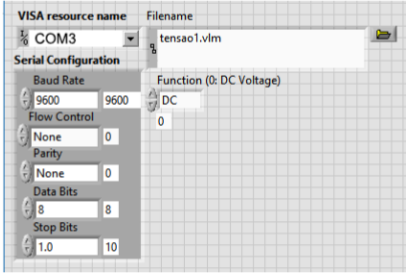
\includegraphics[scale = 0.8]{b.png}
                    \caption{Painel frontal do LabVIEW na avaliação da rede elétrica}
                    \label{frontallv}
                \end{figure}
                
                \begin{figure}[H]
                    \centering
                    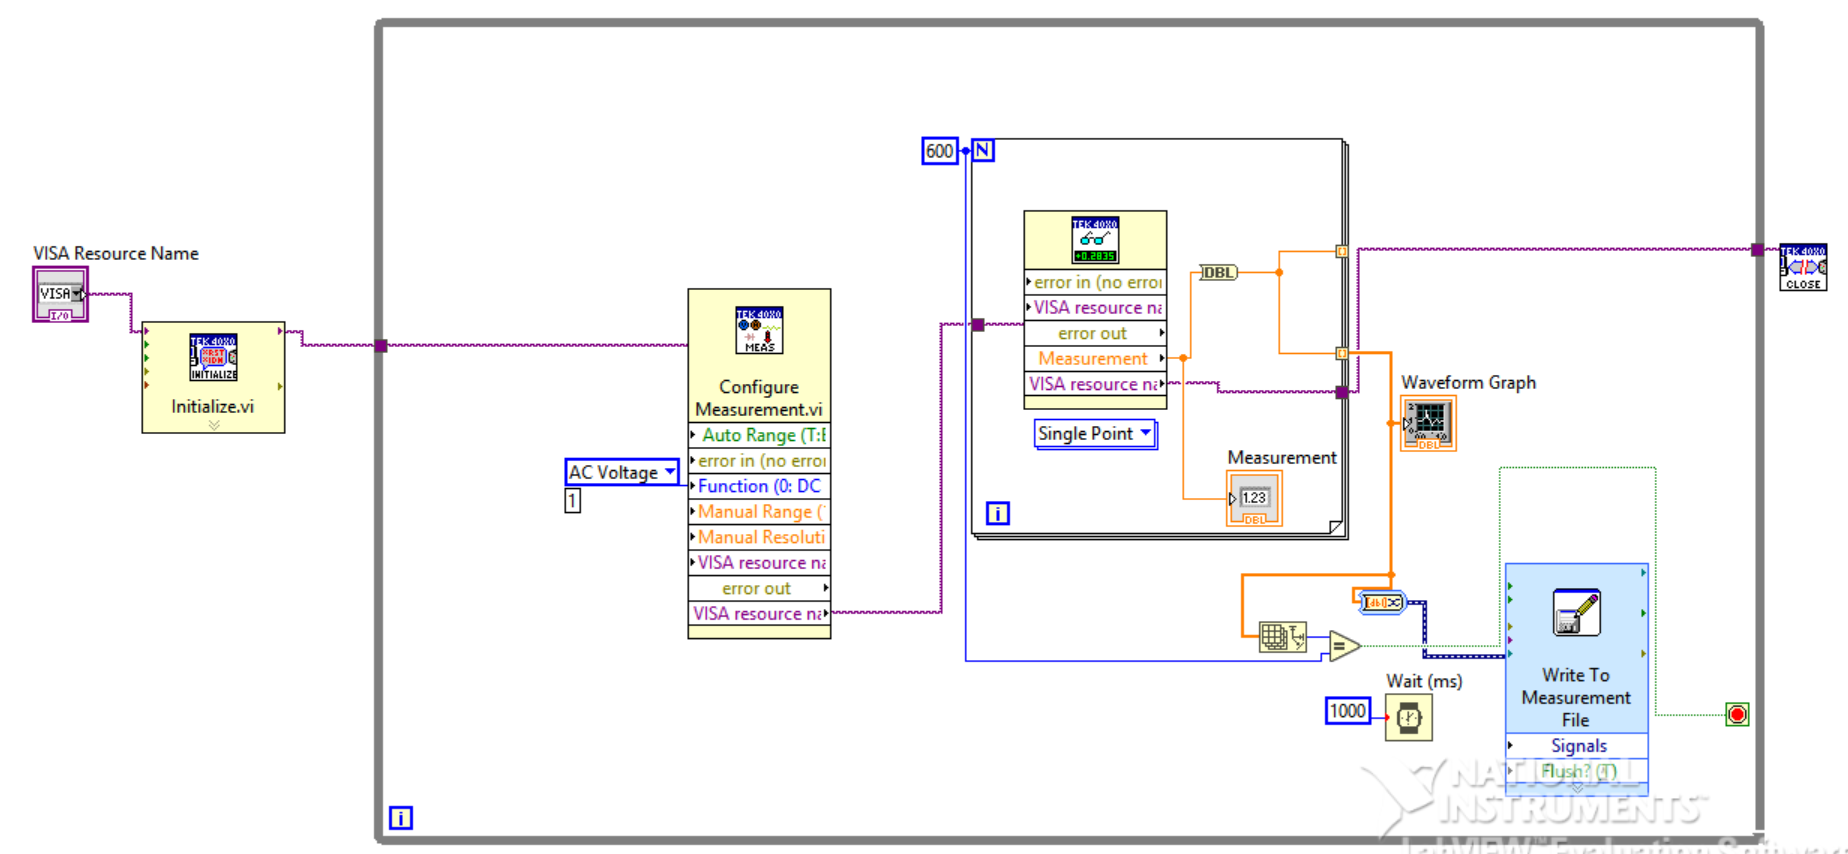
\includegraphics[scale = 0.5]{Labview_rede.PNG}
                    \caption{Diagrama de Blocos do LabVIEW na Avaliação da Rede Elétrica}
                    \label{frontallv}
                \end{figure}
                
               
            
            \section{Avaliação do LM$741$}
                \tab Para fazer análise do amplificador operacional LM$741$, foi usado o multímetro TEKTRONIX DMM4040 para observar a resposta em frequência para as formas de onda senoidal e quadrada, sempre dentro da faixa linear de operação do componente. Disso, as medidas foram realizadas de forma automática, através do esquema do LabVIEW mostrado abaixo.
                \begin{figure}[H]
                    \centering
                    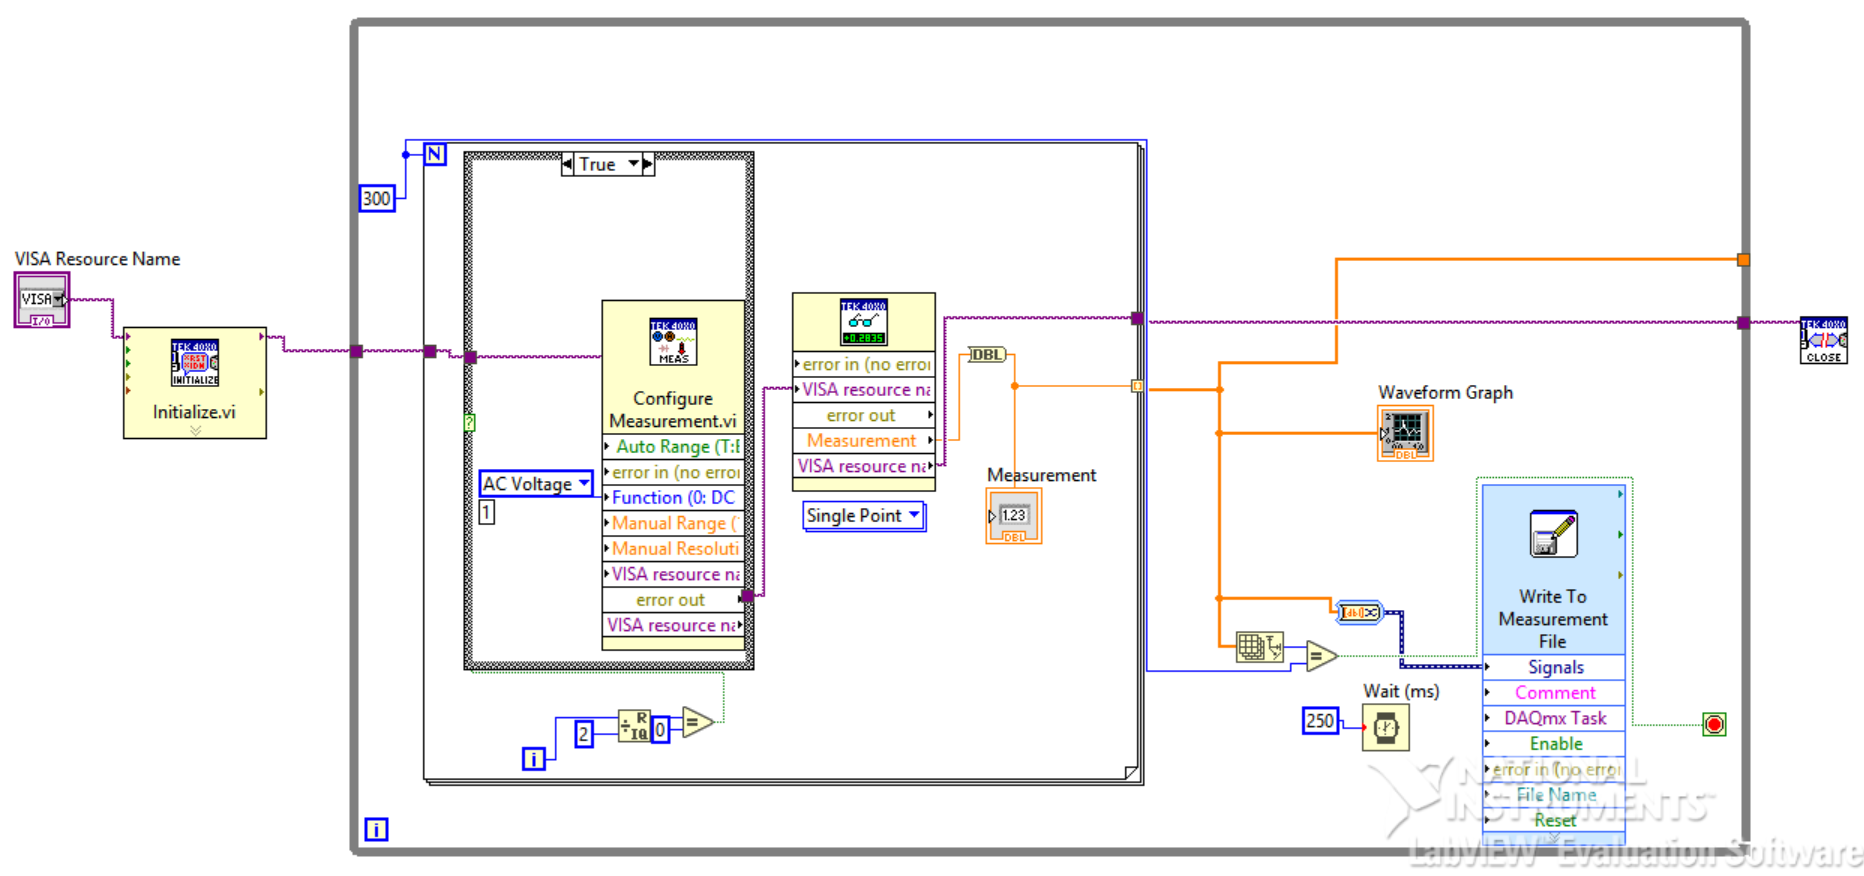
\includegraphics[scale = 0.5]{Labview_amplificador.PNG}
                    \caption{Diagrama de Blocos do LabVIEW na Avalição do LM$741$}
                    \label{labviewampop}
                \end{figure}
                
            \section{Avaliação do Sistema de Medição}
                \tab Para realizar a avaliação do sistema medição como um todo, foi utilizado a placa de circuito ja confeccionada, o multímetro TEKTRONIX DMM4040 e um computador com o software LabVIEW instalado. Para analisar todo um espectro diferenciado de temperaturas, o LabVIEW foi configurado de forma a apresentar, no painel frontal, os valores de medidas realizadas no mensurando em graus Celsius, inicialmente numa temperatura baixa, perpassando pela temperatura ambiente até uma temperatura quente (o mais próxima possível dos 40 graus Celsius) e depois deixar o sistema voltar à temperatura ambiente. \\
                \tab Com o objetivo de ter uma maior segurança na análise final dos dados, tal procedimento é repetido $3$ vezes, o esquema do LabVIEW é mostrado abaixo.
                
                \begin{figure}[H]
                    \centering
                    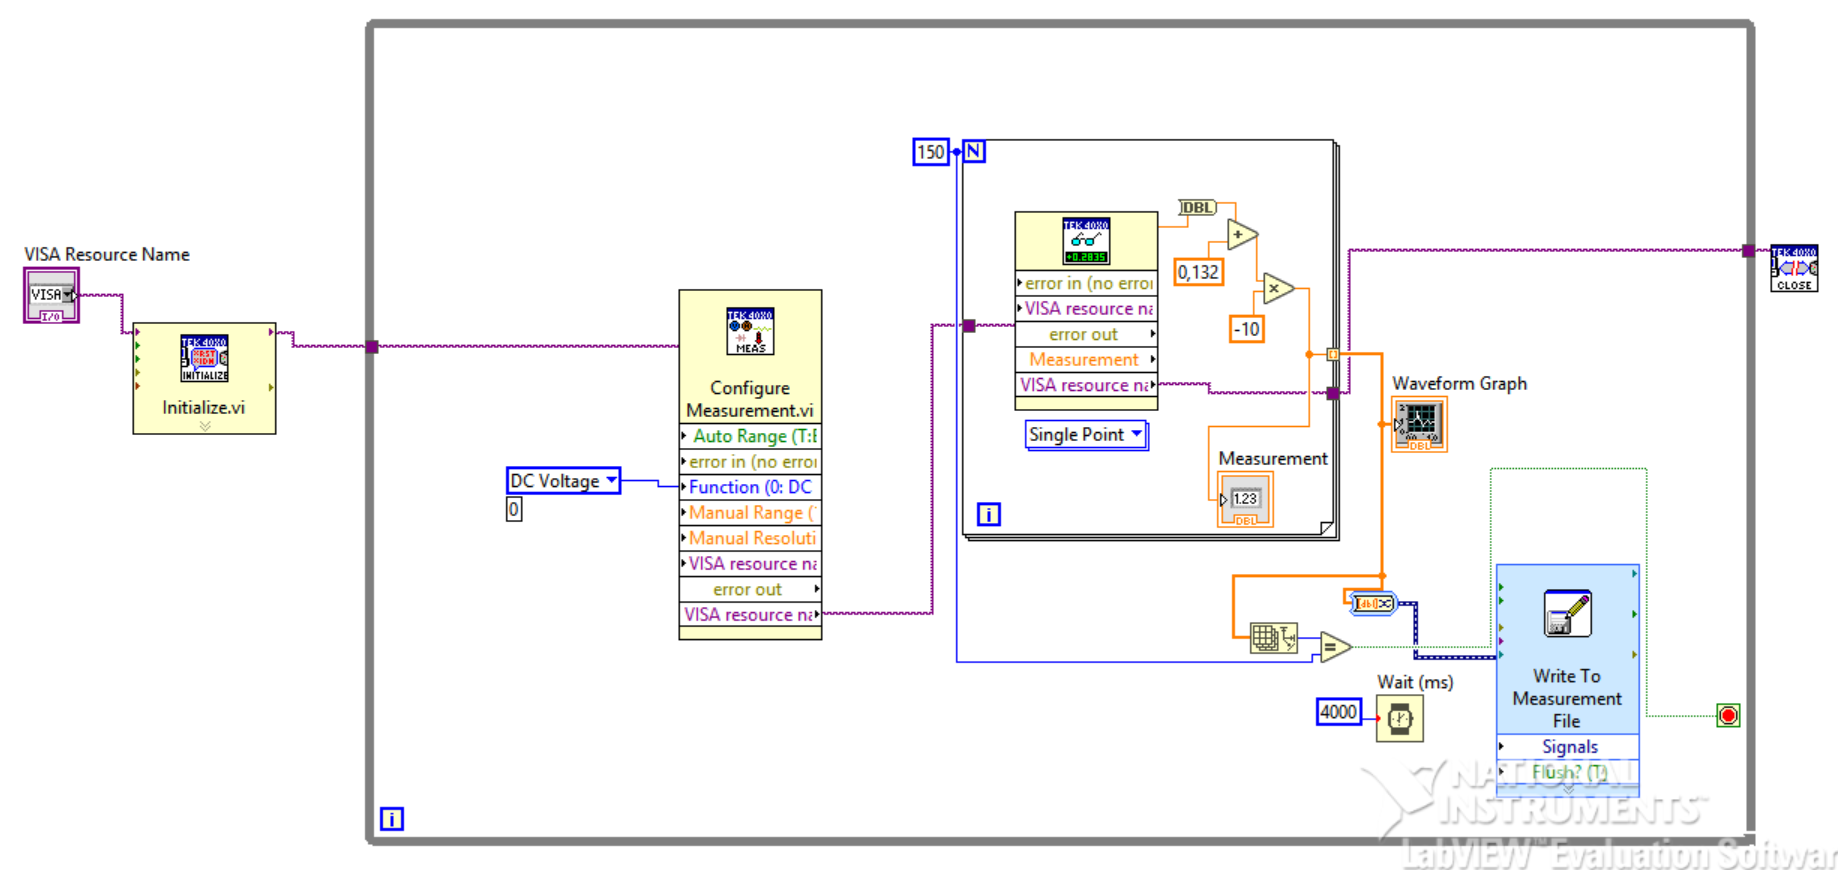
\includegraphics[scale = 0.5]{Labview_temperatura.PNG}
                    \caption{Diagrama de Blocos do LabVIEW na Avalição do Sistema de Medição}
                    \label{labviewmedicao}
                \end{figure}
                
                
                
        \chapter{Desenvolvimento}
        
            \section{Avaliação da Rede Elétrica}
                \tab Utilizando o esquema da Figura 4.3, foi possível obter um total de $600$ amostras, disso, foi elaborado os histogramas abaixo para $3$ momentos diferentes de medição, com os valores da tensão elétrica medida
                
                \begin{figure}[H]
                        \centering
                        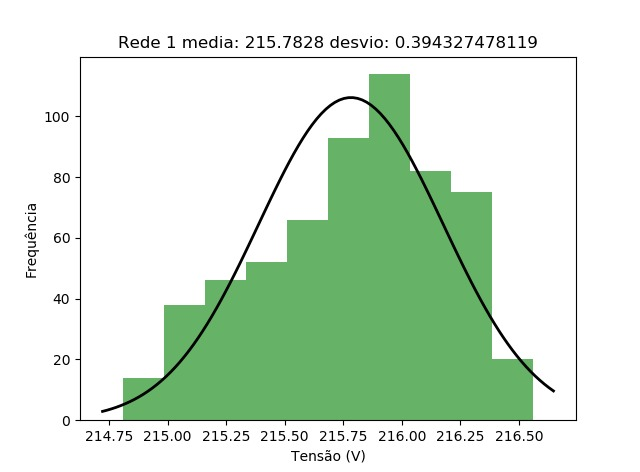
\includegraphics[scale = 0.6]{22.jpeg}
                        \caption{Histograma $1$ de Valores da Tensão da Rede Elétrica}
                        \label{22}
                    \end{figure}
                
                \begin{figure}[H]
                        \centering
                        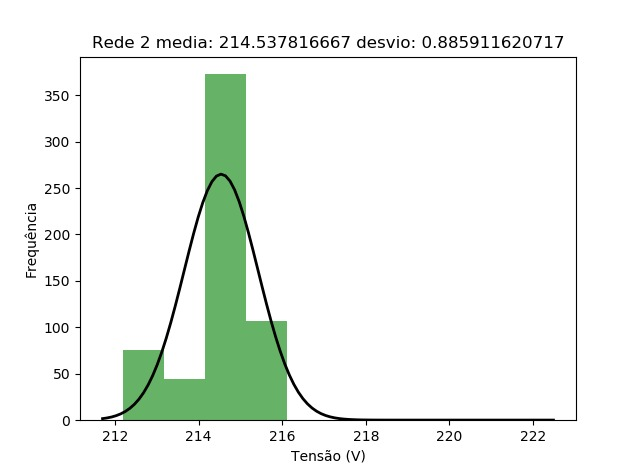
\includegraphics[scale = 0.6]{11.jpeg}
                        \caption{Histograma $2$ de Valores da Tensão da Rede Elétrica}
                        \label{11}
                    \end{figure}
                
                \begin{figure}[H]
                        \centering
                        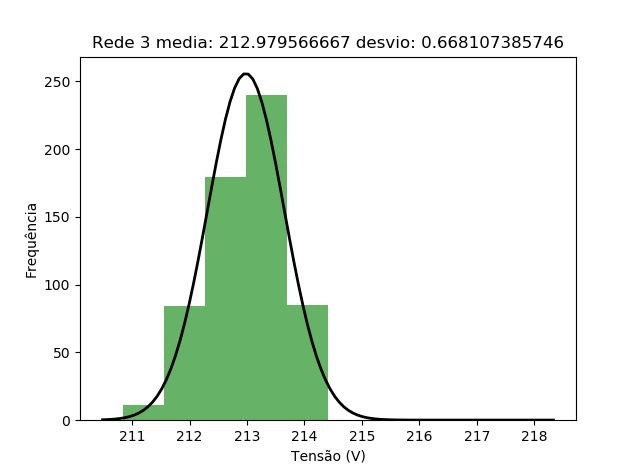
\includegraphics[scale = 0.6]{33.jpeg}
                        \caption{Histograma $3$ de Valores da Tensão da Rede Elétrica}
                        \label{33}
                    \end{figure}
            
          
            
            
            
            \section{Avaliação do LM$741$}
                \tab Com as medidas feitas pelo esquema representado na Figura 4.4, foi possível elaborar os dois gráficos no Excel, sendo um para a resposta em regime de onda senoidal, e o outro para a resposta em regime de onda quadrada, conforme mostrado abaixo
                
                \begin{figure}[H]
                        \centering
                        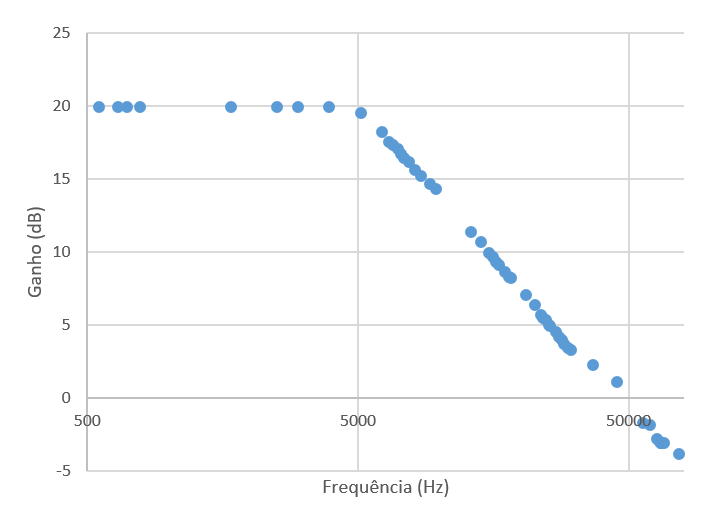
\includegraphics[scale = 1]{amplificacao_senoidal(db).PNG}
                        \caption{Gráfico da Resposta em Frequência para Regime Senoidal LM$741$}
                        \label{senoidal}
                    \end{figure}
                    
                \begin{figure}[H]
                        \centering
                        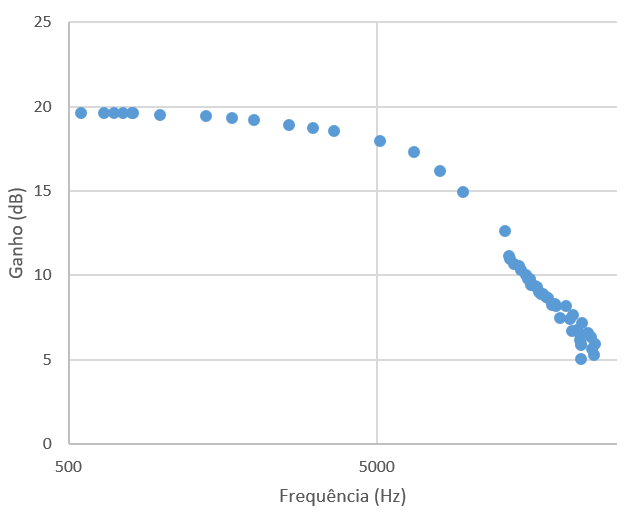
\includegraphics[scale = 1]{amplificacao_quadrada(db)2.PNG}
                        \caption{Gráfico da Resposta em Frequência para Regime Quadrado LM$741$}
                        \label{quadrada}
                    \end{figure}

            \section{Avaliação do Sistema de Medição}
			    \tab Com as medidas feitas pelo esquema representado na Figura 4.5, foi possível elaborar os três gráficos no Excel, sendo cada gráfico a medida da temperatura nas seguintes situações: inicialmente em contato com agua fria, posteriormente sem mensurando especifico (temperatura da sala do laboratório), depois com um ferro de solda ligado próximo ao sensor, e por fim a mercer a temperatura da sala novamente. \\
			    \tab A diferença entre os gráficos é que as medidas foram feitas em momentos diferentes, para se ter uma análise mais segura.
			    
			    \begin{figure}[H]
                        \centering
                        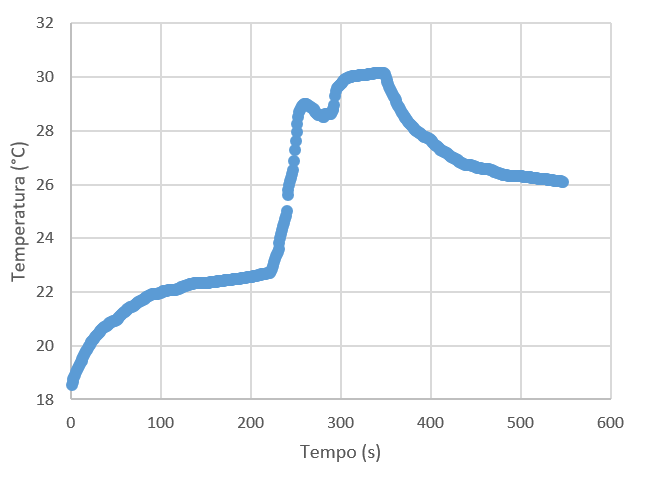
\includegraphics[scale = 1]{1medida_temperatura_x_tempo.PNG}
                        \caption{Primeiro Gráfico de Temperatura x Tempo}
                        \label{primeiro}
                    \end{figure}
                    
                \begin{figure}[H]
                        \centering
                        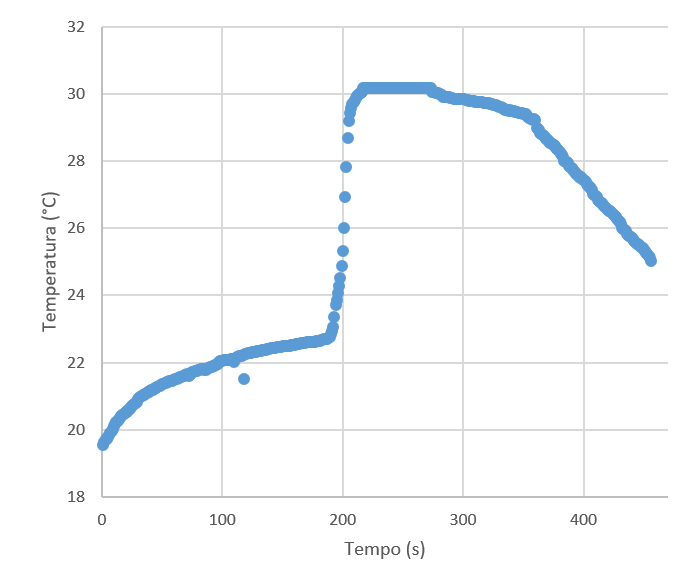
\includegraphics[scale = 1]{2medida_temperatura_x_tempo_certo.PNG}
                        \caption{Segundo Gráfico de Temperatura x Tempo}
                        \label{segundo}
                    \end{figure}
                
                \begin{figure}[H]
                        \centering
                        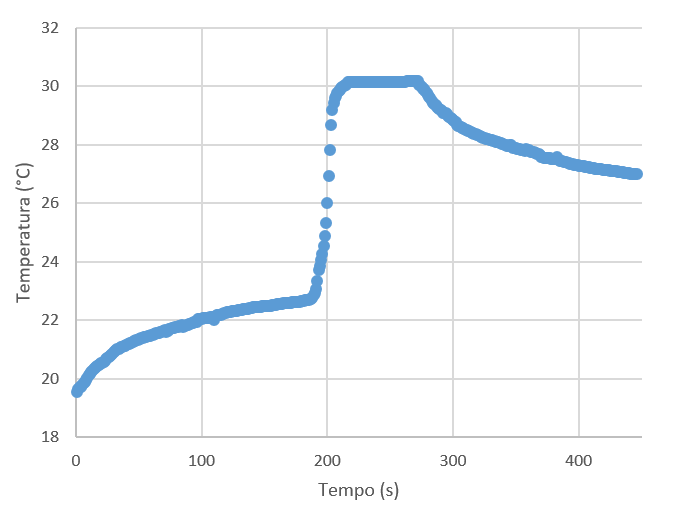
\includegraphics[scale = 1]{3medida_temperatura_x_tempo_certo.PNG}
                        \caption{Terceiro Gráfico de Temperatura x Tempo}
                        \label{terceiro}
                    \end{figure}
            
                
        \chapter{Análise}
            \section{Avaliação da Rede Elétrica}
                \tab Segundo a ANEEL (Agência Nacional de Energia Elétrica), para regiões de tensão nominal 220V, serão permitidas tensões entre 209V e 231V. \\
                \tab De acordo com os dados das Figuras 5.1, 5.2 e 5.3, percebe-se que a tensão da rede elétrica no laboratório está dentro dos padrões estabelecidos. Observa-se que o desvio padrão se manteve baixo, o que condiz com o fato de que nenhuma medição indicou um valor inadequado. \\
                \subsection{Objetivo}
                    \tab Analisar a qualidade da rede elétrica no Laboratório LADAMS do DES.
                \subsection{Métodos utilizados}
                    \tab A fim de verificar a qualidade da rede elétrica mediu-se a tensão em 3 momentos diferentes. Em cada série foram obtidas 600 medições espaçadas igualmente em um período de 10 minutos.
                 \subsection{Conclusão}
                    \tab A tensão entregue a rede elétrica está de acordo com os padrões da ANEEL, logo é adequada para o uso. \\
            
            \section{Avaliação do LM$741$}
                \tab Como observado nas Figuras 5.4 e 5.5, o amplificador possui uma atenuação do ganho menor do que 3dB na faixa de frequência até aproximadamente 7kHz, tanto para a onda quadrada quanto para a senoidal. Valores maiores geram uma distorção na medição.
                \subsection{Objetivo}
                    \tab Avaliar do amplificador operacional LM741.
                \subsection{Métodos utilizados}
                    \tab Foram realizados dois testes para avaliar o ganho real e a resposta em frequência do amplificador operacional utilizado. O primeiro utilizou-se uma onda senoidal e variou-se a frequência. No segundo, foi feito o mesmo teste utilizando uma onda quadrada.
                 \subsection{Conclusão}
                    \tab O sistema de medição está apto para ser utilizado, uma vez que as curvas tiveram um comportamento dentro do esperado. \\
                
            \section{Avaliação do Sistema de Medição}
                \tab Como exposto na seção 5.3, percebe-se que o sistema de medição obteve bons resultados. Verifica-se também a pouca variação das medições, uma vez que os gráficos são bem similares. \\
                \subsection{Objetivo}
                    \tab Avaliar a qualidade do sistema de medição automático de temperatura.
                \subsection{Métodos utilizados}
                    \tab Para a análise do sistema de medição desenvolvido, realizou-se 500 medições de temperatura, em intervalos de 1 segundo, de um determinado mensurando submetido à variações de temperatura. Este procedimento foi repetido três vezes.
                 \subsection{Conclusão}
                    \tab O sistema de medição está apto para ser utilizado, uma vez que as curvas de temperatura tiveram um comportamento semelhante e dentro do esperado. \\
                

        \chapter{Conclusão}
            \tab O desenvolvimento do trabalho foi de extrema importância para a vivência prática dos conhecimentos adquiridos ao longo das aulas da disciplina de Medidas Eletromagnéticas. \\
            \tab Inicialmente verificou-se a importância do uso do software LabVIEW, bastante utilizado no mercado a fora, como software principal para esquematizar medidas automatizadas, visto a quantidade incrível de medidas que se consegue fazer em pouquíssimo tempo, agregando bastante fidelidade aos resultados finais. \\
            \tab Algo bastante relevante no desenvolver do projeto foi o aprendizado relacionado ao uso do software LabVIEW. Durante o processo de instalação, até o primeiro uso efetivo ocorreram problemas, o processo de instalação é bastante complicado e não existe boas documentações na rede. Problemas comuns de acontecer e que, com a vivência do presente projeto, foram resolvidos e absorvidos como forma de conhecimento. \\
            \tab Ocorreu também diversas vezes em que precisamos analisar especificações do fabricante, checar informações no datasheet, prática bastante importante para um engenheiro e que foi feita pela primeira vez no curso através desse projeto e do projeto anterior. \\
            \tab Por fim, apesar das imperfeições, das incertezas de medida e dos desvios de realidade, os resultados finais foram bastante próximos do esperado, de forma que o projeto foi, além de muito importante como forma de conhecimento, um produto final válido.
            
                
                
\end{document}